% Dr. Nam H. Le. drnamlabs.com, bunnyquant.com
\documentclass[11pt]{article}
\usepackage[a4paper,margin=2.4cm]{geometry}
\usepackage[T1]{fontenc}
\usepackage{lmodern}
\usepackage{microtype}
\usepackage{graphicx}
\usepackage{booktabs}
\usepackage{array}
\usepackage{xcolor}
\usepackage{caption}
\usepackage{amsmath}
\usepackage[round,authoryear]{natbib}
\usepackage{tikz}
\usetikzlibrary{positioning,arrows.meta,fit,backgrounds}
\usepackage[colorlinks=true,linkcolor=teal!70!black,urlcolor=teal!70!black,citecolor=teal!70!black]{hyperref}

\graphicspath{{figs/}}
\captionsetup{font=small,labelfont=bf}
\definecolor{ink}{HTML}{1A2B32}
\definecolor{tealx}{HTML}{0F7C86}
\definecolor{amber}{HTML}{C97A1E}
\newcommand{\Vm}{V_\mathrm{mem}}

\title{\textbf{Physics as the Referee}\\[3pt]
\large A biology language model built from scratch and trained against a tissue simulator}
\author{Nam H. Le\\[2pt]
\small Department of Computer Science and Vermont Complex Systems Institute\\
\small University of Vermont, \texttt{nam.le@uvm.edu}}
\date{\small Technical report, October 2026. Not peer reviewed.}

\begin{document}
\maketitle

\begin{abstract}
\noindent
Biomedical language models are trained on text and graded on text, so a
fluent answer and a correct one look the same to every metric in the loop.
Bioelectricity is a domain where this need not be the case, because a
physics simulator can compute what a tissue would do under a described
intervention. We use that simulator as the reward for reinforcement learning
and ask what it changes. To keep every training token under our control, we
built the entire pipeline from scratch: a byte-pair tokenizer and a
40M-parameter transformer pretrained on 0.99 billion tokens of PubMed
cell-biology abstracts, followed by instruction tuning, direct preference
optimization and group-relative policy optimization against the BETSE
bioelectric tissue simulator. On held-out simulator problems the model
reaches a reward of 0.945, higher than the strongest open chat model we ran
locally, even when that model was given five worked examples (0.904). A sealed exam
placed between the training lattice points then cut the score to 0.539 and
showed that the model had mostly learned a lookup table; changing where the
training simulations were placed, with the algorithm and budget fixed,
restored it to 0.777, and in-context examples to 0.835. In a second track we adapt
an open pretrained model to the same corpus and find that domain adaptation
reliably trades away dialogue, through mechanisms we can measure: answer length
inherited from the post-training data, forgetting under LoRA, and two
shortcut cues created by the data mixture. We argue that, at this scale,
language, facts and physical consequences should be held in three different
places (weights, a citable library, and the simulator), and that exam design
decides what a simulator-verified score actually certifies.
\end{abstract}

%======================================================================
\section{Introduction}

Language models are now asked questions about living systems that used to
go to a textbook or a colleague: what a channel blocker does to a cell's
resting potential, why a tissue depolarizes, which intervention might
restore a pattern \citep{singhal2023large,wang2023scientific}. The standard
way to build such a model is to continue pretraining a general model on
biomedical text and then tune it on question--answer pairs
\citep{gururangan2020dont,luo2022biogpt,chen2023meditron,wu2024pmcllama}.
The standard way to test it is a literature-derived benchmark such as
PubMedQA \citep{jin2019pubmedqa}. Both halves of this recipe stay inside
text. Training rewards the model for sounding like the literature, and
evaluation rewards it for agreeing with the literature, which it may have
seen \citep{magar2022data,sainz2023nlp}. No step asks whether a claim would hold in
the tissue it describes.

For most of biology there is no way to ask that question cheaply. For
bioelectricity there is. The voltage across cell membranes ($\Vm$), shaped
by ion channels, pumps and gap junctions, carries patterning information
during development and regeneration \citep{levin2021bioelectric}, and the
BETSE simulator integrates the electrodiffusion equations for whole
tissues of coupled cells \citep{pietak2016exploring}. Given bath
concentrations and channel permeabilities, BETSE returns the steady-state
$\Vm$ that a tissue reaches. A model's statement that a given intervention
depolarizes the tissue to $-21$\,mV can therefore be checked against the
physics, with no annotator involved.

This matters because reinforcement learning with verifiable rewards has
become the main way to teach models skills that imitation cannot
\citep{lambert2024tulu,shao2024deepseekmath,deepseek2025r1}. The verifiers
in that line of work are mostly string checkers for mathematics and code. A
simulator is a different kind of verifier. It does not compare an answer to
a reference that someone wrote down; it computes the outcome. The question
we pursue is what such a verifier buys in a small domain model, and what it
does not.

We built the whole system from scratch, from tokenizer to reinforcement
learning, and ran it on a single consumer GPU. This was a methodological
choice rather than a display of effort. Because we produced every training
token, contamination could be audited instead of assumed away; because we
wrote every stage, each failure could be traced to the stage that caused
it; and because the system is small, every claim here can be re-run in
hours.

The paper makes four contributions. First, it describes a complete
pretraining and post-training pipeline for a 40M-parameter cell-biology
model whose final stage is trained against a tissue simulator, together with
the engineering problems that came up at each stage and how they were
resolved (Sections~\ref{sec:scratch}--\ref{sec:sim}). Second, it shows that
a simulator-verified score on a standard held-out split can overstate what
a model has learned, and that a sealed off-grid exam exposes the gap: the
model had learned a lookup table, and the fix was in the placement of
training data, not in the learning algorithm (Section~\ref{sec:results}).
Third, it reports a controlled study of adapting a pretrained open model to
the same corpus, in which every loss of dialogue ability is traced to a
measurable property of the training data (Section~\ref{sec:trackb}). Fourth,
it argues from these results for a division of labour, in which the weights
carry language, a retrieval library carries facts with citations, and the
simulator carries physical consequences (Section~\ref{sec:discussion}).

%======================================================================
\section{Related work}

\paragraph{Domain language models.} Domain-specific pretraining from
scratch was shown to beat general pretraining for biomedical understanding
by PubMedBERT \citep{gu2021domain}, and generative models followed:
BioGPT \citep{luo2022biogpt} and BioMedLM \citep{bolton2024biomedlm}
trained on PubMed, while BloombergGPT \citep{wu2023bloomberggpt} mixed domain and
general data. The more common route continues
pretraining an open general model \citep{gururangan2020dont}, as in
Meditron \citep{chen2023meditron} and PMC-LLaMA \citep{wu2024pmcllama}, and
then instruction-tunes it, often on answers written by a stronger model.
Our Track A is a from-scratch model in the BioGPT tradition but far
smaller, chosen by the compute-optimal ratio for our corpus
\citep{hoffmann2022training}; Track B is the continued-pretraining route
run on a small open base \citep{allal2025smollm2}.

\paragraph{Post-training and verifiable rewards.} Instruction tuning
\citep{wei2022finetuned} and preference learning from human feedback
\citep{ouyang2022training} turned pretrained models into assistants. Direct
preference optimization removed the separate reward model
\citep{rafailov2023direct}, and group-relative policy optimization (GRPO)
removed the value network \citep{shao2024deepseekmath}. Training on rewards
computed by a program, rather than learned from preferences, has driven
recent gains in reasoning \citep{lambert2024tulu,deepseek2025r1}, with
verification also applied at the level of steps \citep{lightman2023verify}. We
implement SFT, DPO and GRPO ourselves and replace the program verifier with
a physics simulator. The over-optimization we observed with DPO matches the
reward hacking reported by \citet{gao2023scaling}.

\paragraph{Evaluation and contamination.} Benchmark overlap with
pretraining data inflates scores \citep{magar2022data,sainz2023nlp}.
Likelihood-based multiple-choice scoring is sensitive to the prior over
answer strings \citep{zhao2021calibrate,holtzman2021surface}, which turned
out to be central to our PubMedQA result. LAB-Bench \citep{laurent2024labbench}
tests research-style biology tasks and was out of scope for a
512-token text model.

\paragraph{Forgetting and shortcuts.} Sequential training on new data
erodes earlier abilities
\citep{mccloskey1989catastrophic,kirkpatrick2017overcoming}, including
in large language models under continual fine-tuning \citep{luo2023empirical}.
Replaying earlier data mitigates this \citep{ibrahim2024simple}, and LoRA
\citep{hu2022lora} learns less and forgets less than full fine-tuning
\citep{biderman2024lora}. Models also latch onto incidental features that
correlate with labels \citep{gururangan2018annotation,geirhos2020shortcut};
we document two such cues that our own data mixture created. The view that
post-training mostly teaches format \citep{zhou2023lima}, and the finding
that imitation transfers style more readily than capability
\citep{gudibande2023false}, frame our Track B results.

\paragraph{Retrieval and long-tail facts.} Small models recall rare facts
poorly \citep{kandpal2023large,mallen2023when}, which motivates
retrieval-augmented generation \citep{lewis2020retrieval}. Our library
uses classical full-text ranking \citep{robertson2009probabilistic} with a
reader trained only on sentences mined from the corpus.

\paragraph{Language models in discovery loops.} FunSearch
\citep{romera2024mathematical} and AlphaEvolve \citep{novikov2025alphaevolve}
pair a language model that proposes candidates with an automatic evaluator
that scores them, and quality-diversity search \citep{mouret2015illuminating}
keeps the candidate pool varied. The simulator loop described here is the
evaluator half of such a system for bioelectricity.

%======================================================================
\section{System overview}

The system has a model in the middle and two components that tie it to the
domain (Figure~\ref{fig:pipeline}). The first is the corpus, 3.2 million
PubMed abstracts, which serves as pretraining data and, through a full-text
index, as a library the model can quote with PubMed identifiers (PMIDs). The second is the
verifier: BETSE, which scores numeric predictions about tissue voltage.
Everything between these two components is generic. Track A fills the
middle with a model trained from random initialization; Track B fills it with
an open pretrained model and keeps the corpus, verifier and exams fixed, so
that the two tracks differ mainly in their starting weights. A web
application, public at \url{https://drnamlabs.com/cellbio/}, runs the loop
in front of the user: one specifies an intervention, the model predicts
mean $\Vm$, BETSE runs, and the prediction is marked against the simulated
tissue.

\begin{figure}[t]
\centering
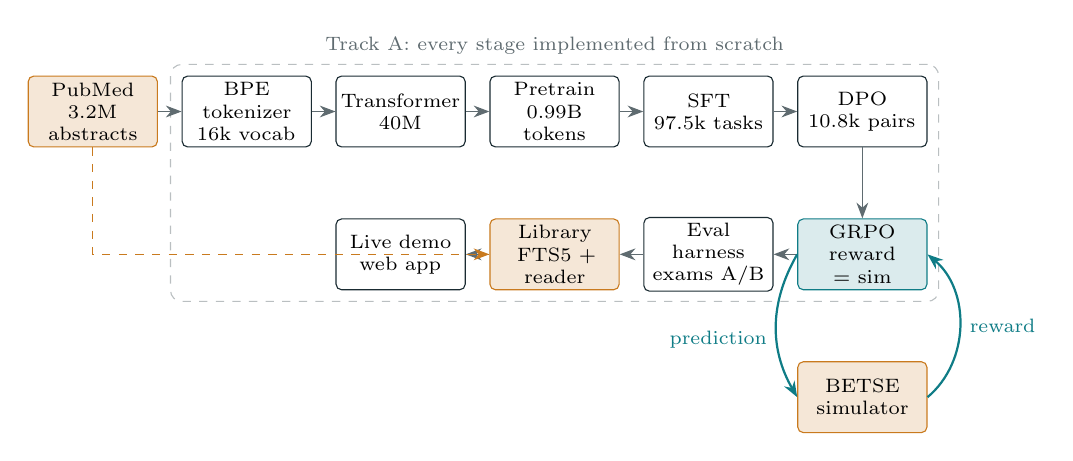
\begin{tikzpicture}[
  node distance=3mm and 3mm,
  st/.style={draw=ink,rounded corners=2pt,fill=white,font=\scriptsize,
             minimum height=9mm,text width=15mm,align=center,inner sep=2pt},
  sock/.style={st,fill=amber!18,draw=amber},
  rl/.style={st,fill=tealx!15,draw=tealx},
  ar/.style={-{Stealth[length=2mm]},draw=ink!70}]
\node[sock] (data) {PubMed\\3.2M abstracts};
\node[st,right=of data] (tok) {BPE tokenizer\\16k vocab};
\node[st,right=of tok] (tf) {Transformer\\40M};
\node[st,right=of tf] (pt) {Pretrain\\0.99B tokens};
\node[st,right=of pt] (sft) {SFT\\97.5k tasks};
\node[st,right=of sft] (dpo) {DPO\\10.8k pairs};
\node[rl,below=9mm of dpo] (grpo) {GRPO\\reward = sim};
\node[sock,below=9mm of grpo] (betse) {BETSE\\simulator};
\node[st,left=of grpo] (eval) {Eval harness\\exams A/B};
\node[sock,left=of eval] (lib) {Library\\FTS5 + reader};
\node[st,left=of lib] (demo) {Live demo\\web app};
\foreach \a/\b in {data/tok,tok/tf,tf/pt,pt/sft,sft/dpo,dpo/grpo,grpo/eval,eval/lib,lib/demo}
  \draw[ar] (\a) -- (\b);
\draw[ar,tealx,thick] (betse.east) to[bend right=50] node[right,font=\scriptsize,text=tealx]{reward} (grpo.east);
\draw[ar,tealx,thick] (grpo.west) to[bend right=30] node[left,font=\scriptsize,text=tealx,pos=.6]{prediction} (betse.west);
\draw[ar,amber,dashed] (data.south) |- (lib.west);
\begin{scope}[on background layer]
\node[draw=ink!30,dashed,rounded corners,fit=(tok)(dpo)(grpo)(demo),inner sep=4pt,
      label={[font=\scriptsize,text=ink!70]above:Track A: every stage implemented from scratch}] {};
\end{scope}
\end{tikzpicture}
\caption{Pipeline. The amber components (corpus and library, simulator)
tie the system to the domain; the rest is generic. Track B keeps the amber
components and the exams and replaces the from-scratch transformer with an
open pretrained model.}
\label{fig:pipeline}
\end{figure}

%======================================================================
\section{Building the model from scratch}
\label{sec:scratch}

All runs used seed 42 and a single RTX 5090 shared with other jobs, so
every process was capped at 30\,GB of GPU memory and 12 CPU threads.
Checkpoints, logs, metrics and sample generations were written to disk at
every stage, and failed runs were kept. Table~\ref{tab:hparams} in the
appendix lists the hyperparameters.

\subsection{Corpus}
We selected PubMed records under the MeSH headings Morphogenesis,
Regeneration, Cell Physiological Phenomena and Tissue Engineering, with
NCBI's own hierarchy expansion, keeping only records with an abstract. A
validation pass on one baseline file gave a 5.0\% in-domain yield and 516
tokens per document, which suggested a corpus of about 1.7B tokens. The
full fetch ran into three undocumented behaviours of the E-utilities
service. Retrieval through a stored result set stops after the first
10{,}000 records, so we split the query by entry date, bisecting any date
range that still exceeded the cap, which gave 482 slices. The service
sometimes returns HTTP 200 with truncated XML, so fetching and parsing were
retried together, and a slice that kept failing was logged without stopping
the run. Rate-limit replies come back as valid JSON without a result count,
so a missing count was treated as a retry signal. The final corpus has
3,198,416 documents (1.6\,GB compressed, no failed slices, no duplicate
PMIDs). Its word count, 616M, corrected the earlier projection to roughly
0.8--1.0B tokens. Because the parameter count was chosen from the token
count, this correction moved the model from a planned 80--100M parameters
down to 40M. The five most recent slices are held out as a temporal
validation set, so all validation text was published after all training
text.

\subsection{Tokenizer and architecture}
The byte-pair encoder \citep{sennrich2016neural} was written from scratch
and trained on the corpus with 16,384 tokens. It compresses the text to 4.91
bytes per token and keeps domain terms such as \emph{depolarization} and
\emph{regeneration} as single tokens. Round-trip encoding is exact. The
model is a decoder-only transformer \citep{vaswani2017attention,radford2019language}
in plain PyTorch, without library transformer modules: 10 layers, 8 heads,
width 512, context 512, rotary position embeddings \citep{su2024roformer},
RMSNorm \citep{zhang2019root}, SwiGLU feed-forward blocks
\citep{shazeer2020glu} and tied input and output embeddings
\citep{press2017using}, for 40.5M parameters. Before any real training we
checked the implementation three ways. A single batch was overfit from loss
9.77 to 0.049 in 68 steps. A hand-written attention agreed with PyTorch's
fused kernel to $2.4\times10^{-6}$. Generation with the key--value cache
matched full recomputation token for token.

\subsection{Pretraining}
The model was trained for one epoch over 988.5M tokens: 30,167 steps of
32,768 tokens with AdamW \citep{loshchilov2019decoupled}, a peak learning
rate of $6\times10^{-4}$ with 500 warmup steps and cosine decay, and bf16
autocast. The run took 62 minutes. We stopped at one epoch because the
compute-optimal ratio was already met \citep{hoffmann2022training} and
repeated data gives diminishing returns \citep{muennighoff2023scaling}.
Temporal-validation loss fell from 9.70 at initialization to 2.436
(perplexity 11.4), and training and validation loss stayed together
throughout (Figure~\ref{fig:pretrain}). Samples went from token soup
to fluent methods prose about patch clamping and ATPase kinetics, with invented
details.

\begin{figure}[t]
\centering
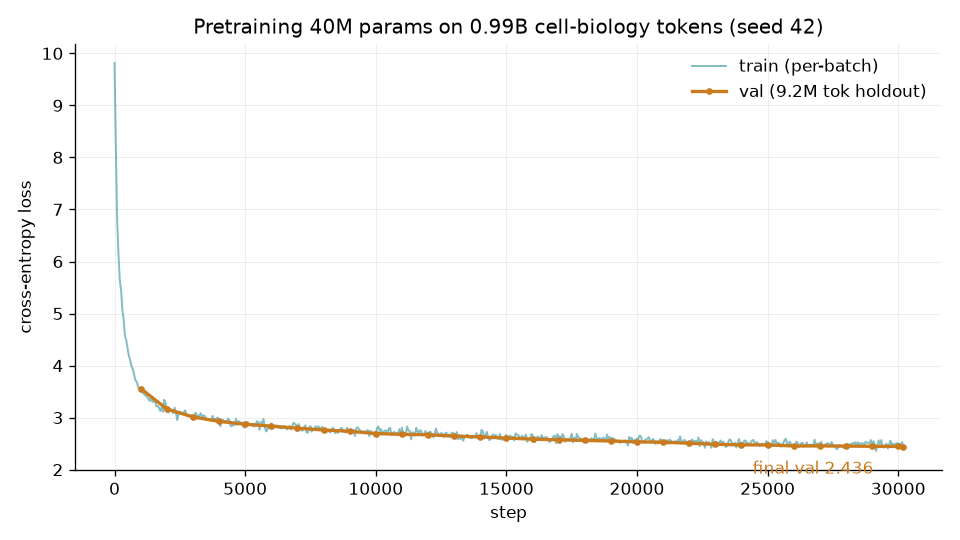
\includegraphics[width=.62\linewidth]{loss_curve.png}
\caption{Pretraining loss of the 40M model on the training stream and the
temporal hold-out.}
\label{fig:pretrain}
\end{figure}

\subsection{Instruction tuning}
We wanted the from-scratch track to contain no text written by another
model, so instruction data was mined from the corpus. Four tasks were
extracted from abstracts in the training slices: titles phrased as questions
paired with the abstract's conclusion, ``$X$ is a\dots'' sentences turned
into definitions, abbreviations paired with their expansions, and title
generation. This gave 97.5k examples. Loss was computed on answer tokens
only. Two epochs at learning rate $6\times10^{-5}$ took about five minutes
and brought masked validation loss to 2.316. The model switched from
continuing text to answering it. One
failure was systematic: the model answered ``ATP stands for ATP''. Common
abbreviations are almost never spelled out in abstracts, so the
abbreviation task never showed their expansions, and the model learned to
copy.

\subsection{Preference optimization}
DPO \citep{rafailov2023direct} was implemented from the loss formula, using
masked sequence log-probabilities under the policy and a frozen copy of the
SFT model. At step zero the two models are identical and the loss must
equal $\ln 2$, which it did. We mined 10,841 preference pairs without an external model.
The chosen answer was the gold answer. The rejected answer was either the SFT
model's own sample at temperature 0.8 or a circular hard negative of the
form ``$X$ stands for $X$''. The first run ($\beta=0.1$, learning rate
$5\times10^{-6}$, all tasks) eliminated circular answers but raised the
four-gram repetition rate from 0.27 to 0.46, and answers drifted off topic. We traced
this to two causes: a loose KL constraint, and noisy chosen answers in the
question-title task, where the abstract's last sentence does not always
answer the title. The second run kept only the definition and abbreviation
tasks, raised $\beta$ to 0.3 and lowered the learning rate to
$2\times10^{-6}$. Circular answers fell from 4.4\% to 0.0\% on held-out
prompts and repetition was unchanged (0.272 to 0.276). The ATP answer
stopped being circular but was still wrong. Preference optimization can
redistribute probability among answers the model can already produce; it cannot supply a fact the
model never saw.

\subsection{Reinforcement learning against an equation}
Before using the simulator we tested the RL machinery on a verifier that
could not be wrong: the Nernst equation, the single-ion law that BETSE
integrates. A generator produced three families of problems: the numeric
equilibrium potential in millivolts, the direction of change when a
concentration moves, and the polarity of the resulting shift. These were
split 85/15 by parameter combination, so held-out combinations never
appeared in training. The reward parser gives full credit within 2\,mV and
partial credit within 10 and 25\,mV; every gold answer must score 1.0, and a
self-test enforces this. GRPO \citep{shao2024deepseekmath} was implemented
with 16 prompts and 8 samples per step, advantages normalized within each
group, a token-level policy-gradient loss and a KL penalty of 0.05 against
the starting model. Two practical points decided whether it worked at all.
Starting from the SFT model, most groups received the same low reward
and gave no gradient; 400 steps of supervised warm start on the problem
format fixed this. Groups in which all samples received the same
reward carry no signal and were skipped. Over 300 steps (7.5 minutes),
training reward rose from 0.72 to 0.87. The categorical families
generalized perfectly, but held-out numeric reward moved only from 0.565 to
0.599, while KL rose to 0.22. The model memorized the combinations it had
been trained on and did not learn the logarithm.

%======================================================================
\section{The simulator as verifier}
\label{sec:sim}

\subsection{Running BETSE inside the training pipeline}
BETSE 1.5.0 fails on Python 3.13, so it runs in a separate Python 3.11
environment and the training code calls it as a subprocess. Two settings
caused errors that the simulator does not report clearly. Custom ion
concentrations are silently ignored unless the ion profile is set to
\texttt{custom}, and the intracellular and extracellular ion sets must each
be electrically neutral or the run aborts. We therefore raised
extracellular K$^+$ by lowering Na$^+$ by the same amount, as in a
high-potassium Ringer's solution. On a 213-cell tissue, one configuration
takes about 13\,s from seeding to per-cell $\Vm$ readout. As a first check,
raising bath K$^+$ from 5 to 25\,mM depolarized the tissue from $-43.8$ to
$-20.7$\,mV, as expected.

The language model never talks to BETSE during training
(Figure~\ref{fig:interface}). We ran 150 simulations offline, eight in parallel, over
a grid of ten bath K$^+$ levels, five K$^+$ permeability multipliers
(0.25--4) and three Na$^+$ permeability multipliers (0.5--2). This took 6.8
minutes with no failures. Mean $\Vm$ spans $-74.9$ to $-7.2$\,mV, and the
slice at four times K$^+$ permeability is non-monotone in bath K$^+$, an
effect of multi-cell coupling with no closed form. Each simulation became
text problems that ask for the steady-state mean $\Vm$ or the direction of
the shift, giving 466 training and 98 held-out problems. The split was made
by hashing the knob combination, so no held-out combination was ever
simulated for training. The reward uses the same bands as the Nernst stage.

\begin{figure}[t]
\centering
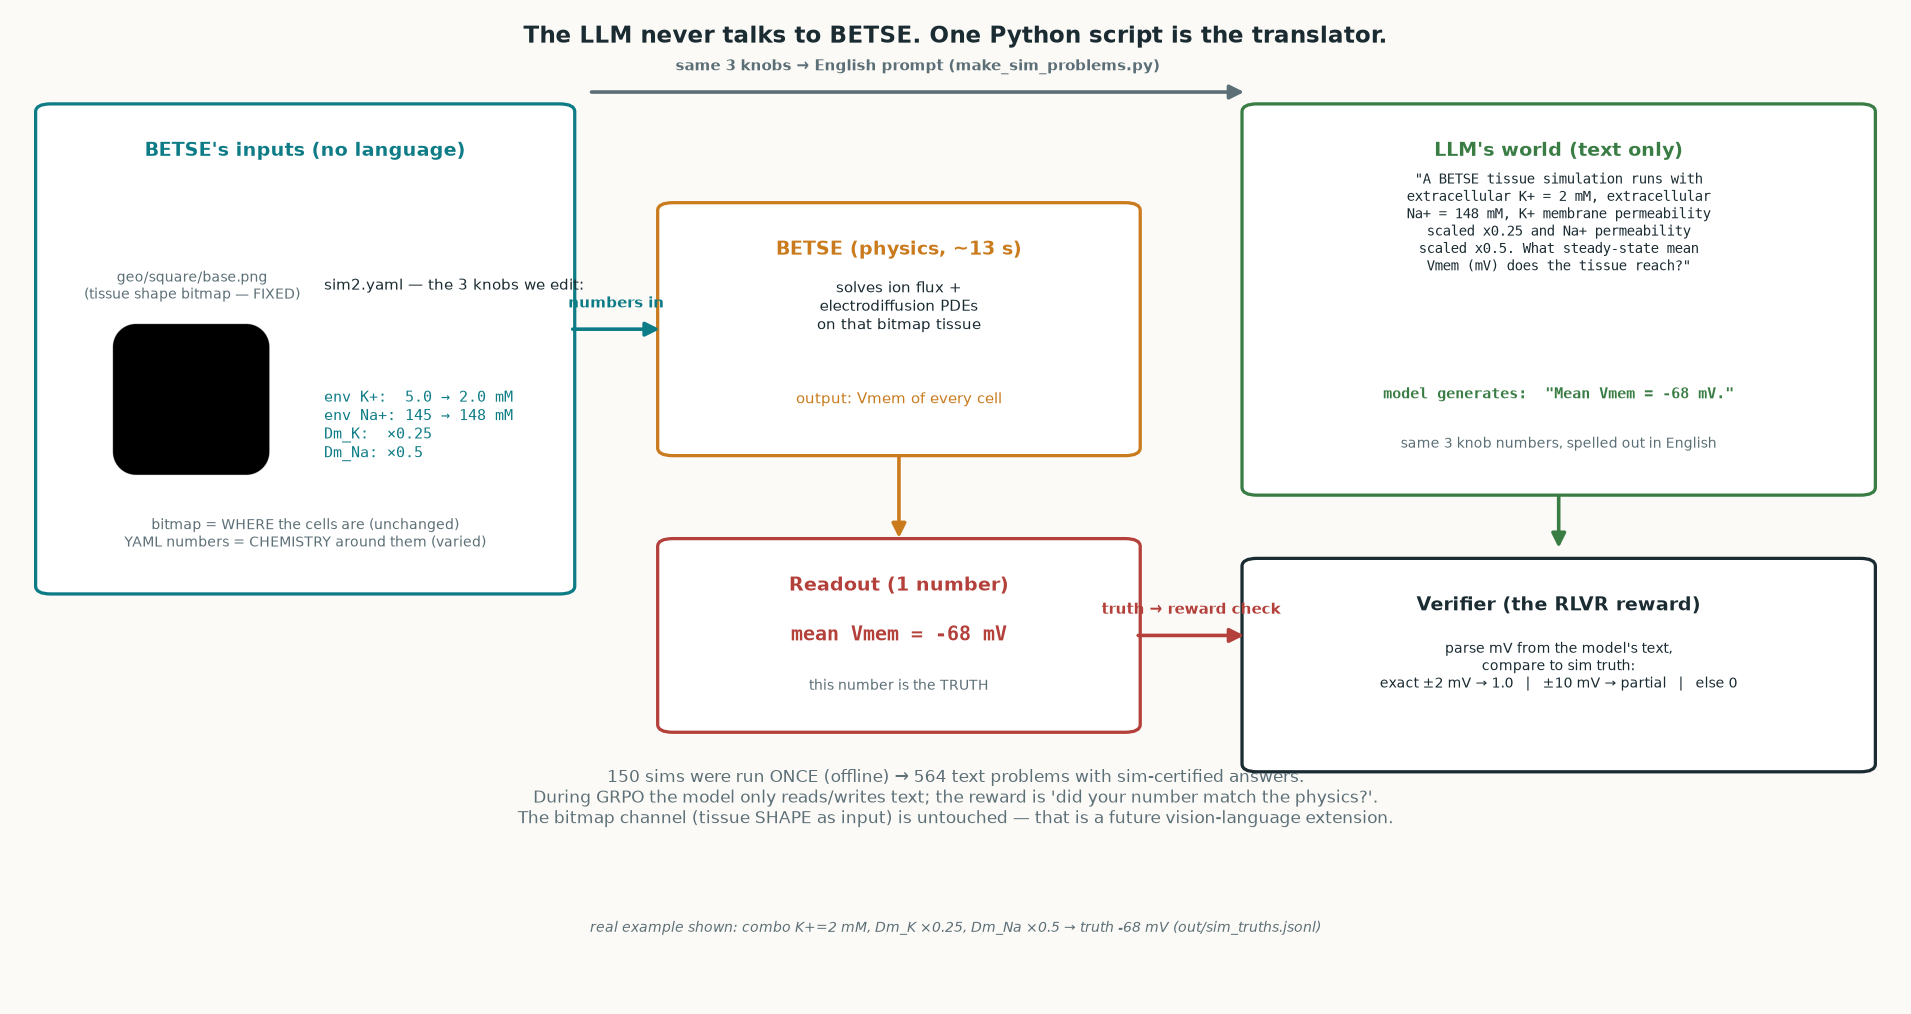
\includegraphics[width=\linewidth]{explain_interface.png}
\caption{How the simulator becomes a reward. Interventions are simulated
once and turned into text problems, and the model's numeric answer is
parsed and scored against the simulated tissue.}
\label{fig:interface}
\end{figure}

\subsection{Training}
Starting from the textbook model, 300 steps of supervised warm start on
training gold answers were followed by 200 steps of GRPO with the same
settings as before, with 60\% of each batch drawn from numeric problems.

\subsection{A second exam, and a change of training data}
The 98 held-out problems hide lattice \emph{nodes}, not \emph{regions}:
every test point has trained neighbours one grid step away. To test
generalization we built exam B from 60 new simulations at decimal knob
values drawn log-uniformly inside the grid range, each at least 0.25 in
$\log_2$ units (median 0.43) from every training node. This gave 234
problems, which were sealed before any model was scored on them. When the
lattice-trained model failed this exam (Section~\ref{sec:results}), we
asked whether the cause was the learning algorithm or the training data.
We spent the same budget of 150 simulations on knob values drawn at random
over the same range, each kept at least 0.2 $\log_2$ units from every
exam-B point, and retrained with an identical recipe. A third variant added five
nearest training examples, with their simulated $\Vm$, as text in the
prompt, the same five-shot condition we gave the pretrained baselines. A
first attempt at this failed: a model warm-started only on bare questions
treated the examples as noise, and its accuracy fell when they were
present. Warm-starting on a mixture with zero to five examples per prompt
taught the model to use them.

%======================================================================
\section{Evaluation methodology}
\label{sec:eval}

One harness scores every checkpoint on the same exams: perplexity on the
temporal hold-out, PubMedQA \citep{jin2019pubmedqa}, the 727 held-out
textbook problems, and simulator exams A and B. PubMedQA is built from
PubMed abstracts, so we checked it against our corpus: 59 of its 1,000
labelled items share a PMID with our training data. All PubMedQA scores
are reported both on the full set and on the 941 clean items, and the two never differ by more than 1.1
points. Multiple-choice answers are scored by length-normalized
log-probability of each option, which needs no answer parsing.

We compare against two kinds of reference. The first is a set of floors: chance, and
a constant predictor that always gives the most common training answer
for each problem type. The constant predictor scores 0.538 on exam A
because the partial-credit bands reward a central guess, so it must always
be reported. The second is a set of six open-weight chat models served locally, each
given the same strictly formatted prompt with zero or five worked examples.
One of them first scored 0.17. Reading its transcripts showed that it had
written all of its output into a separate reasoning channel and left the
answer field empty. After the harness was fixed to read the correct field,
it scored 0.455 zero-shot and 0.664 five-shot. Since then we read raw
transcripts before reporting any external model's score.

A second evaluation bug came from our own code. The library reader first
scored a token-F1 of 0.39 on held-out questions. The batched evaluation
had left-padded prompts, but the model had never seen padding and had no
attention mask. Grouping prompts of equal length into the same batch, with no padding, raised the
score to 0.990 with no change to the model. All batched generation in the
project now groups prompts by length this way.

%======================================================================
\section{Retrieval library}

The library is a SQLite FTS5 index over titles and abstracts of all 3.2M
documents (8.2\,GB, five minutes to build). Retrieval first requires all
query terms and falls back to any of them, with a small synonym map and a
rerank that favours sentences of the form ``\emph{term} is a \emph{noun}''.
A reader was trained on 29,054 examples mined the same way as the SFT data,
with a definition sentence as the answer and its surrounding abstract as
context. In free generation the 40M reader stitched fragments together
when the context lacked a clean definition. We therefore changed the
mechanism from generation to selection. Candidate sentences are extracted
from the retrieved abstracts, the reader ranks them by likelihood, and the
best sentence is returned verbatim with its PMID. If no candidate exists,
the library declines to answer. Questions that are not definitional are
declined outright, because an off-topic quotation proved worse than no
answer.

%======================================================================
\section{Results}
\label{sec:results}

\begin{table}[t]
\centering\small
\begin{tabular}{@{}lcccc@{}}
\toprule
& Pretrained & +SFT & +DPO & +GRPO (textbook)\\
\midrule
Temporal-holdout perplexity $\downarrow$ & 11.50 & 14.59 & 14.59 & 16.24\\
PubMedQA accuracy (majority class 0.552) & 0.537 & 0.491 & 0.496 & 0.460\\
\quad clean subset (941 items) & 0.526 & 0.480 & 0.486 & 0.453\\
Textbook physics reward (727 held-out) & 0.000 & 0.239 & 0.238 & 0.977\\
\bottomrule
\end{tabular}
\caption{The Track A ladder on three exams it was not trained on.}
\label{tab:ladder}
\end{table}

\paragraph{The training ladder.} Each post-training stage bought a
specific behaviour and paid for it in perplexity (Table~\ref{tab:ladder}).
The textbook RL stage took held-out physics reward from 0.24 to 0.977, while
perplexity on future abstracts rose from 11.5 to 16.2. On PubMedQA every
checkpoint scored below the majority class. All four checkpoints chose
``no'' on zero of 1,000 items, which led us to test three explanations
(Figure~\ref{fig:evals}). Tokenization was ruled out. With an empty prompt, the model
assigned ``no'' about 7 nats less log-probability than ``yes'' ($-13.5$ against
$-6.4$). No training stage had ever produced a yes/no answer, so the
score measured that prior, and the prior happened to mimic the majority
class. Calibrating by the empty-prompt score \citep{zhao2021calibrate}
allowed the model to choose ``no'', but accuracy fell to chance (0.34--0.47),
and removing the abstract entirely moved raw accuracy only from 0.537 to
0.519. The model was not reading the evidence. We report the 0.46--0.54 range
as an artifact of the prior, not as partial competence.

\begin{figure}[t]
\centering
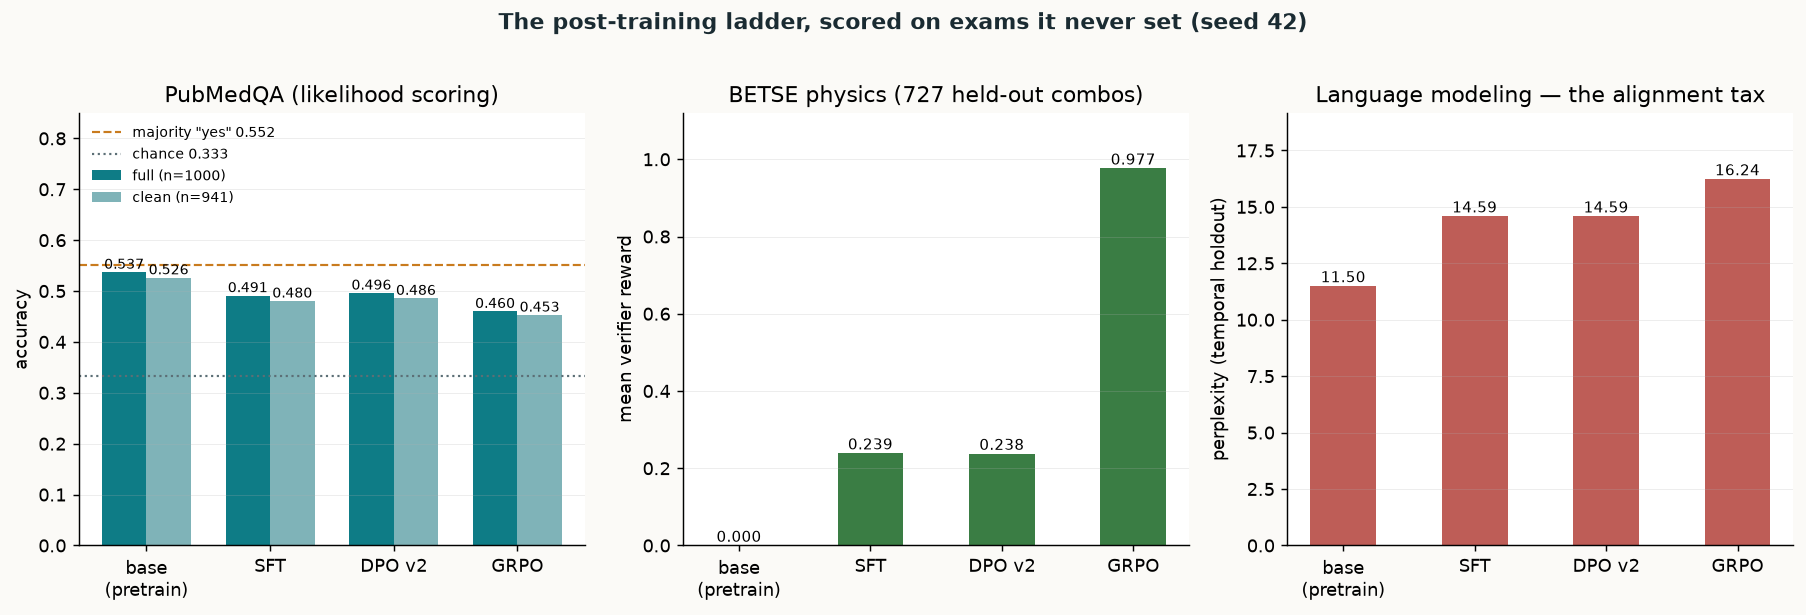
\includegraphics[width=\linewidth]{eval_results.png}\par\vspace{4pt}
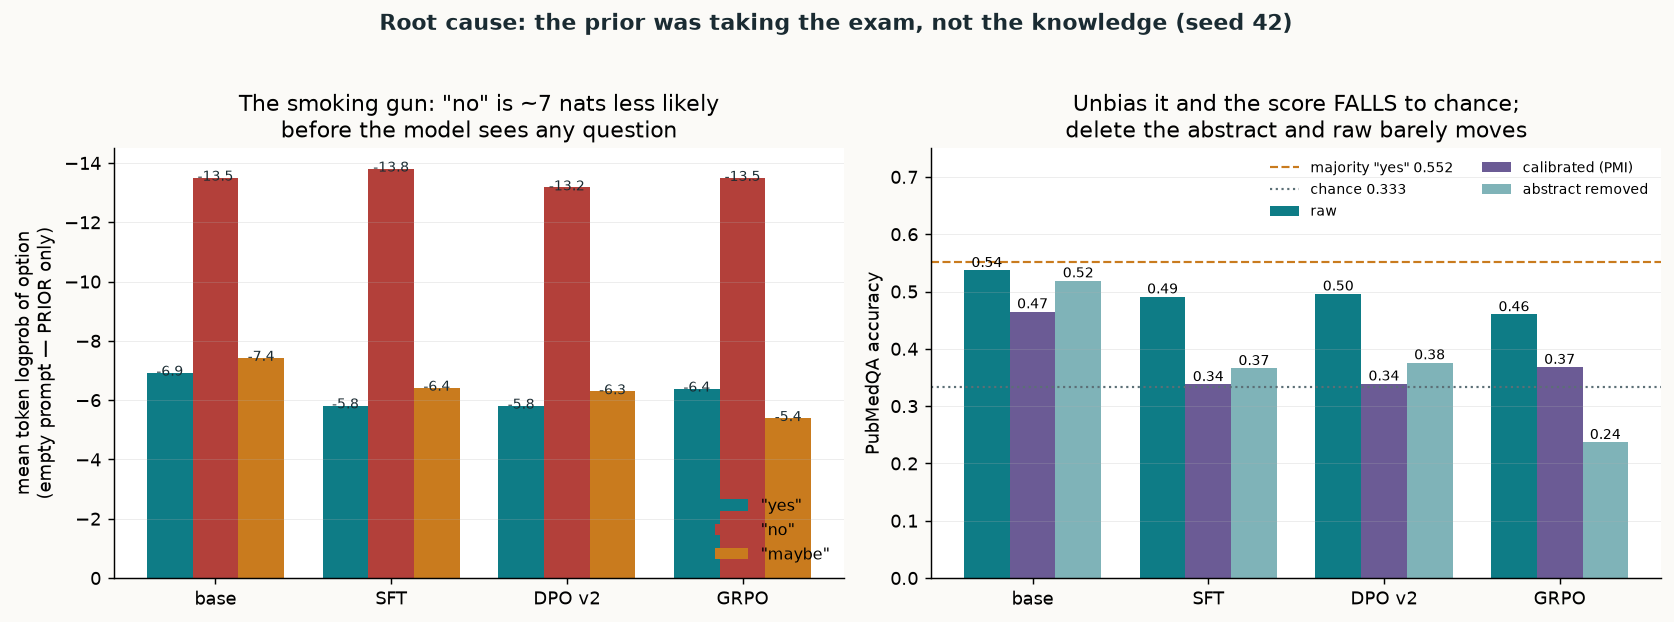
\includegraphics[width=.85\linewidth]{pubmedqa_diagnosis.png}
\caption{Top: the ladder on each exam. Bottom: the PubMedQA diagnosis. An
empty prompt already prefers ``yes'' by about 7 nats, and removing the
abstract barely changes accuracy.}
\label{fig:evals}
\end{figure}

\begin{table}[t]
\centering\small
\begin{tabular}{@{}lcc@{}}
\toprule
& Reward & Numeric only\\
\midrule
\multicolumn{3}{@{}l}{\emph{Exam A: 98 held-out lattice combinations}}\\
Constant predictor & 0.538 & 0.454\\
Own ladder, zero-shot (best checkpoint) & 0.321 & 0.150\\
Best open chat model, zero-shot & 0.529 & 0.216\\
Best open chat model, five worked examples & 0.904 & 0.852\\
Hosted model as agent, zero-shot & 0.562 & 0.462\\
Hosted model as agent, five worked examples & 0.955 & 0.952\\
40M, simulator warm start & 0.938 & 0.898\\
40M, simulator warm start + GRPO & \textbf{0.945} & \textbf{0.912}\\
\midrule
\multicolumn{3}{@{}l}{\emph{Exam B: 234 sealed off-grid problems}}\\
Constant predictor & 0.663 & 0.559\\
40M trained on the lattice & 0.539 & 0.535\\
40M trained on 150 random points, same budget & 0.777 & 0.657\\
\quad + five nearest worked examples in the prompt & \textbf{0.835} & \textbf{0.711}\\
Hosted model as agent, zero-shot & 0.591 & 0.453\\
Hosted model as agent, five worked examples & 0.808 & 0.742\\
\bottomrule
\end{tabular}
\caption{Simulator exams. All rows use the same verifier and the same reward bands.}
\label{tab:sim}
\end{table}

\paragraph{Simulator exams.} On exam A the simulator-trained model scored
0.945, and 0.912 on numeric problems alone (Table~\ref{tab:sim}). Every
generic checkpoint of our own ladder scored zero, because none could
produce the answer format; the textbook RL model reached 0.321. The
strongest open chat model scored 0.529 zero-shot, below the constant
predictor, and 0.904 with five worked examples. The supervised warm start
did most of the work (0.938), and GRPO added a little on top.

\paragraph{A hosted model as an agent.} We also had a hosted frontier LLM
sit the exams as an agent (closed book). The agent read one
question file and wrote one answer file; it could reason before answering
but had no access to the simulator or the truth files, and the same verifier
scored its answers. In a first single test it scored 0.562 on exam A, close
to the constant predictor, and 0.591 on exam B, below it. With the five
nearest worked examples it scored 0.955 on exam A, level with the 40M model
(0.945; 98 problems, so the gap is one problem) and 0.808 on exam B, below
the 40M model's 0.835. Four of those ten batches had to be repeated because
the agent reported using code, against the rules; the discarded attempts
scored within 0.03 of the repeats.

That test could not say whether the gaps were real, so we built exam C
before running anything further: twenty batches of fresh simulations
(300 simulations, 1,146 problems), at points at least 0.25, 0.20 and 0.15
log$_2$ units from every lattice node, random-training point and exam B point.
The plan and the SHA-256 hash of each sealed file were published before any
model or agent saw a batch. Each batch is one unit, so comparisons are paired
over 20 batches (Table~\ref{tab:examc}). The comparison fixed in advance was
the 40M model with five examples against the hosted agent with five examples.
The agent was ahead by 0.045 (95\% bootstrap interval over batches 0.025 to
0.065, Wilcoxon $p=0.0014$) and won 17 of 20 batches, so the near-tie of the
first test did not hold. With five examples the agent also beat nearest-neighbour
lookup (+0.025, $p=0.003$), which the 40M model did not (--0.020, $p=0.015$).
Zero-shot the order reverses: the agent scored 0.106 below the constant predictor
and the 40M model trained on random points 0.063 above it. We read that as the
weights holding part of the simulator's response surface while the agent needs
the examples to reach it.

A second round added a smaller hosted agent and four open models run
through Ollama with greedy decoding and one-line answers (gpt-oss:20b,
Qwen 3.5, Qwen 3.6 and DeepSeek-R1 8B). Their systems and comparisons were
declared before they ran, and the plan records that the zero-shot column was
made the headline after the first-round results were seen. Zero-shot, the
40M model trained on random points (0.772) is ahead of every hosted and open
model, and all of those are below the constant predictor. Given five
examples, the large hosted models gain 0.25 to 0.27 and lead the table (large
agent 0.852, small agent 0.842; the two cannot be told apart, $p=0.37$); the open models
gain 0.10 to 0.33, with Qwen 3.5 (0.784) and Qwen 3.6 (0.759) above the
constant predictor and gpt-oss:20b (0.616) and DeepSeek-R1 8B (0.431) below it.
The 40M model with five examples is 0.035 below the small agent (Holm-adjusted $p=0.02$)
and 0.048 above Qwen 3.6 (Holm-adjusted $p=0.04$). DeepSeek-R1 always reasons
before answering and was given 3,000 tokens; 679 of its 1,146 zero-shot answers
(59\%) and 563 with examples (49\%) were cut off before a final line and score
zero, so its rows measure the token budget as much as the model. The 40M models
were trained on this task and the hosted and open models were not, so the
comparison is not like for like. Only the first comparison was the planned
test; the rest are descriptive, with Holm adjustment over the whole secondary
family. The limits are one run per batch, open models at default quantization,
and tool use by the hosted agents that could be checked only through their own
reports, none of which reported a breach on exam C. GPT and Gemini have not
sat exam C, so it stays sealed.

\begin{table}[t]
\centering\small
\begin{tabular}{@{}lcc@{}}
\toprule
System & Zero-shot & Five examples\\
\midrule
Hosted agent, large & 0.602 & \textbf{0.852}\\
Hosted agent, small & 0.569 & 0.842\\
40M, trained on random points & \textbf{0.772} & --\\
40M, mixed warm start & 0.678 & 0.807\\
40M, trained on the grid & 0.500 & --\\
Qwen 3.5 & 0.465 & 0.784\\
Qwen 3.6 & 0.429 & 0.759\\
gpt-oss:20b & 0.511 & 0.616\\
DeepSeek-R1 8B (truncated) & 0.278 & 0.431\\
Constant predictor & 0.708 & 0.708\\
Nearest-neighbour lookup (diagnostic) & -- & 0.827\\
\bottomrule
\end{tabular}
\caption{Exam C: mean reward over 20 sealed batches (1,146 problems). The 40M
models were trained on this task; the others were not.}
\label{tab:examc}
\end{table}

Exam B changed the reading of these numbers (Figure~\ref{fig:exams}). The
lattice-trained model dropped to 0.539, below the constant predictor. Its
predictions explained the failure: across all 234 problems it produced 17
distinct values, 16 of them answers it had memorized from training, and its
predictions correlated with the true $\Vm$ (0.52) barely more than with
the answer at the nearest training node (0.47). It had learned a
soft lookup table, and exam A, where every test point sits next to a
trained node, could not tell the difference. Moving the same 150 simulations
to random positions raised the off-grid score to 0.777. Predictions now
tracked the truth (correlation 0.59) more closely than the nearest node
(0.50), although the model still emitted only values it had seen in
training. Five worked examples in the prompt raised the score to 0.835.
GRPO on top of that model lowered the off-grid score to 0.812, and the
mixed-example warm start cost zero-shot performance (0.666 against 0.777).
Both costs come from the same recipe that produced the best score.

\begin{figure}[t]
\centering
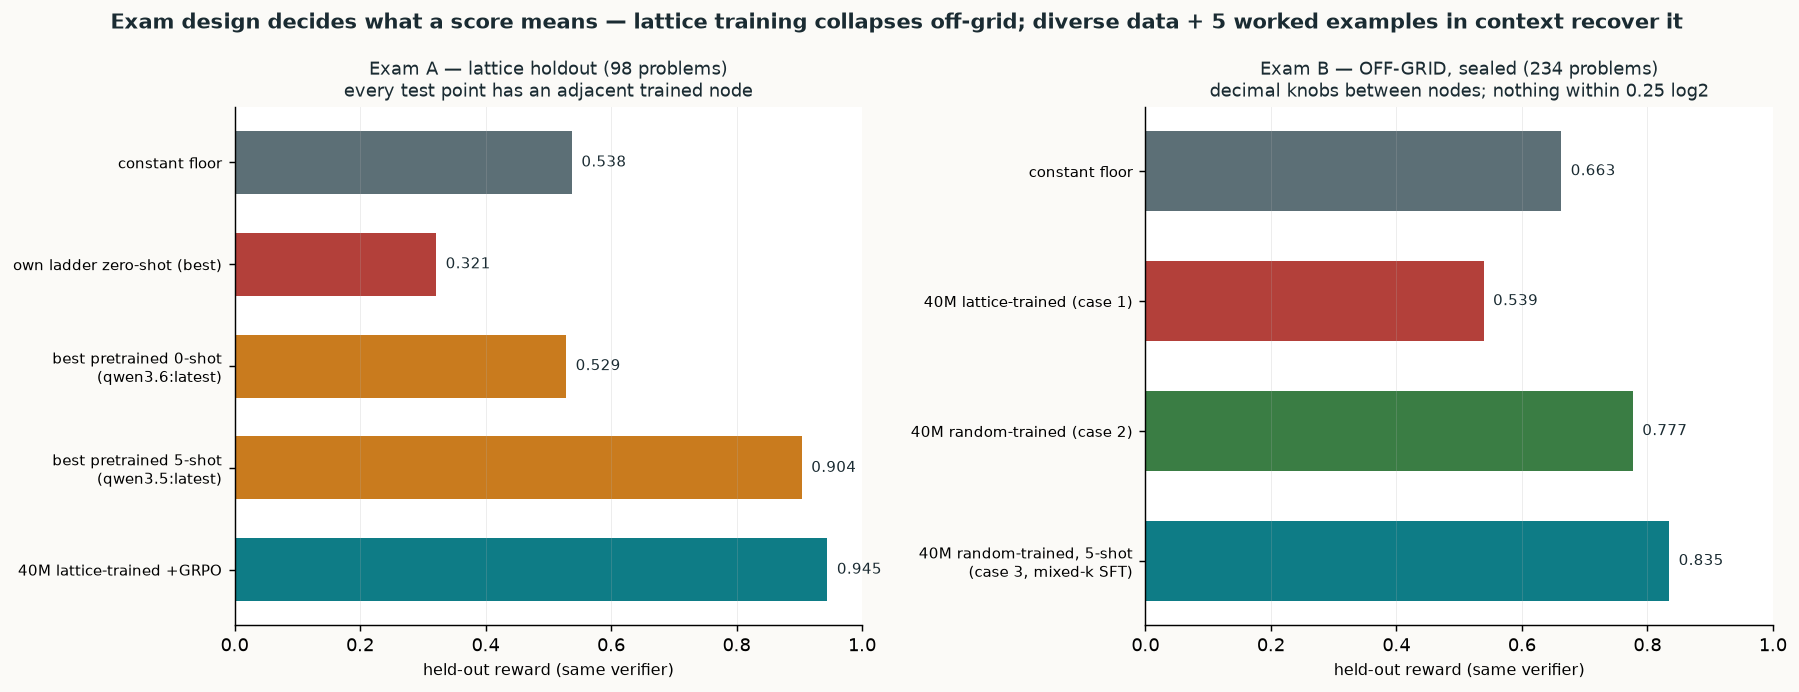
\includegraphics[width=\linewidth]{two_exams.png}
\caption{Exam A against the sealed off-grid exam B. The same model that
leads exam A falls below the constant predictor on exam B; changing where
the training simulations are placed recovers most of the loss.}
\label{fig:exams}
\end{figure}

\paragraph{Library.} On 946 held-out definition questions the reader
reached token-F1 0.990, exact match 0.957, and 0.962 of answers were
verbatim substrings of the retrieved source.

%======================================================================
\section{Adapting a pretrained model}
\label{sec:trackb}

Track A answers simulator problems well but cannot hold a conversation,
write a paragraph or combine sources. Its context is 512 tokens and its
training answers are single sentences. Track B asks whether starting from a
model that already has those abilities, and adding the domain, gives
both.

\subsection{Setup and engineering}
We first tried Qwen2.5-0.5B \citep{qwen2024qwen25}. Its 152k-token
vocabulary made the output logits about 5\,GB per micro-batch of eight
sequences. This ran out of memory beside other jobs, so we used micro-batches of two with sixteen
accumulation steps, which gave 16.5k tokens per second and an 18-hour
epoch. Untouched, this model compressed future PubMed text slightly worse
than our 40M model (0.714 against 0.698 bits per byte). We stopped the run
and switched to SmolLM2-135M \citep{allal2025smollm2}, whose size is close
to Track A's, so that the comparison changes mostly the starting point.
Because the two tokenizers differ, per-token loss is not comparable, and
we report bits per byte on the same temporal hold-out. The corpus took
1.06B tokens under SmolLM2's tokenizer. Full-parameter continued
pretraining ran at 63.8k tokens per second, taking 4.6 hours for one
epoch. For the LoRA route ($r=64$ on all linear layers, 19.5M trainable
parameters) throughput was 53.6k tokens per second. The GPU was 89\% busy
and the CPU 3\%. Keeping the frozen base in bf16 gained only 2\%. Doubling the
micro-batch ran out of memory, because the 49k-vocabulary logits dominate
activation memory, and graph compilation was not available on this platform.

\subsection{Continued pretraining}
Full-parameter continued pretraining took the base model from 0.825 to
0.640 bits per byte and passed Track A's 0.698 after about 131M tokens
(Figure~\ref{fig:routes}). Most of the gain came in the first quarter of
the epoch. LoRA on the instruction-tuned model reached 0.758 after 65M
tokens and 0.677 after the full epoch.

\begin{figure}[t]
\centering
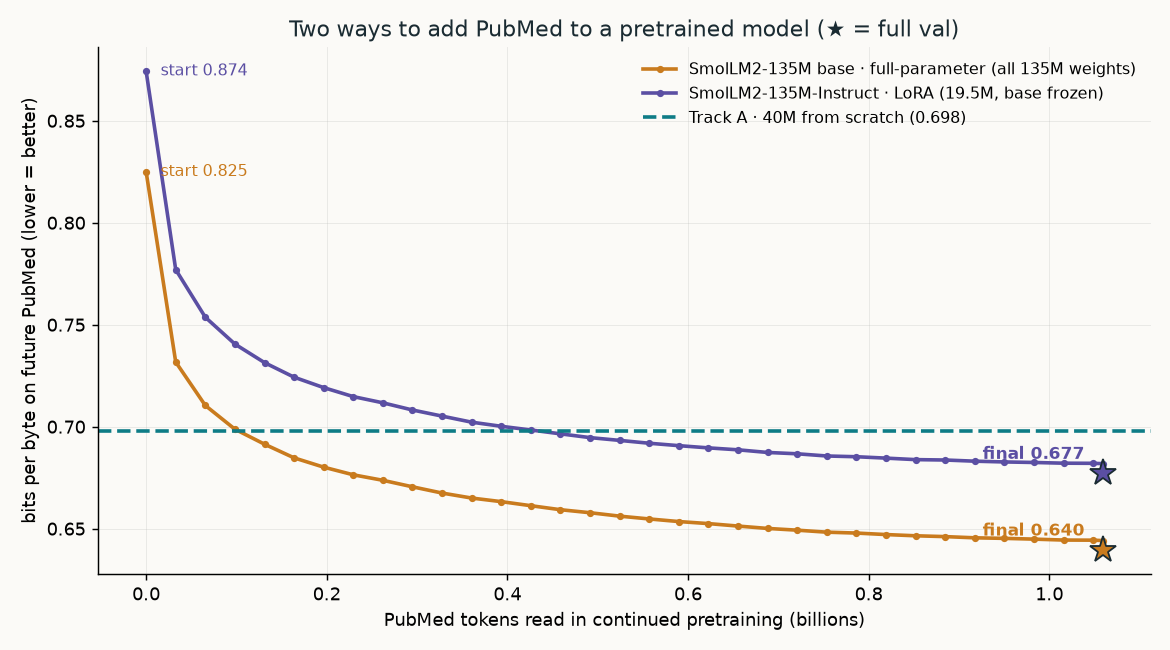
\includegraphics[width=.78\linewidth]{cpt_routes.png}
\caption{Held-out bits per byte during continued pretraining of
SmolLM2-135M, full-parameter on the base model and LoRA on the instruct
model, with Track A's from-scratch model as reference.}
\label{fig:routes}
\end{figure}

\subsection{What happened to dialogue}
Lower bits per byte did not produce a better assistant, and each failure
traced back to the data. After continued pretraining the base model
echoed questions instead of answering them, as Track A had before its SFT
stage. SFT on Track A's 97.5k tasks taught the format but produced answers
of 14--18 words. The SFT answers had a median length of 15 words, and the
model learned when to stop from that distribution; the generation length
limit is only a ceiling. LoRA did not preserve the instruct model's
behaviour either. After one epoch, answers no longer ended on their own,
slid into paper register (``In this article, we will discuss\dots''), ran
into the title of an imagined next abstract and repeated phrases
\citep{holtzman2020curious}. LoRA forgot less than full fine-tuning
\citep{biderman2024lora}, but it still forgot.

We then post-trained the continued-pretraining model on a mixture in the chat template:
80k multi-turn conversations from smol-smoltalk \citep{allal2025smollm2},
whose answers have a median of 187 words and were themselves written by larger
models; 30k long domain examples mined from
training abstracts; and 20k of Track A's short tasks. Loss was applied to every assistant
turn. Self-termination went from 0\% to 100\% of probe answers, but domain
answers stayed short. The cause was in our data. Our system prompt
appeared on every domain example and on no general example, so it had
become a mode switch. With it, the model gave 12--58-word answers in paper
register. Without it, the model gave 173--196-word structured answers that
were generic and wrong (``bioelectricity is electrical stimulation
therapy''). We then drew the system prompt for every example from the same
distribution: none, ours, or a generic one. The switch disappeared, and the
topic took over its role. Biology questions got short paper-style answers
with or without a system prompt (median 32 and 21 words), follow-up
requests to explain more repeated the previous sentence, and one answer
claimed that doubling extracellular K$^+$ doubles the membrane potential.
In the mixture, biology questions were answered only in abstract style, and
long conversational answers occurred only on other topics. No example
showed a biology question answered as a long explanation, so the model had
no way to learn that combination. These are shortcut features in the sense
of \citet{geirhos2020shortcut}, created by how the mixture was assembled.
Domain chat models usually get the missing examples from human writers or
from a stronger teacher model \citep{ouyang2022training,mukherjee2023orca,wu2024pmcllama}.
The mixture also cost domain fit (0.644 to 0.695 bits per byte), the
forgetting that replay is meant to prevent \citep{ibrahim2024simple}.

\paragraph{Reference at 1.5B.} Qwen2.5-1.5B-Instruct, untouched, scored
below the constant predictor on both simulator exams (0.427 and 0.377).
It wrote 150--170-word answers and followed three-turn dialogue, but stated
an invented resting-potential equation with confidence. LoRA SFT on our own
task data alone raised its scores to 0.914 and 0.839 with fluency
intact. Its free-form explanations stayed unsourced and partly wrong. This
model saw both the lattice and random training sets, so its exam-B score is
not directly comparable with Track A's.

%======================================================================
\section{Discussion}
\label{sec:discussion}

\paragraph{The verifier made the small model competitive on the task it
checks.} A 40M model trained against the simulator outscored
general models many times its size on the same numeric problems. The advantage came from the training signal, not from size or
cleverness. The same model, asked an open question, produces fluent
abstract-style prose with invented details, and on PubMedQA its score
reflects a prior, not reading. Simulator training made the model reliable
on the problems the simulator scores and nowhere else.

\paragraph{The exam decides what the verifier certifies.} Exam A used a
standard held-out split and was scored by real physics, yet it rewarded a
lookup table. Only an exam built to fall between training points showed
this, and the remedy was a change in where training simulations were
placed. For anyone building verifier-trained scientific models, this means
that having a physical referee does not remove the need to design the
exam. A held-out split that shares the training lattice measures
memorization, however rigorous the referee.

\paragraph{Where knowledge should live.} Both tracks gave confident wrong
statements whenever a fact had to come from the weights, as reported for
long-tail facts in much larger models \citep{kandpal2023large,mallen2023when}.
Track B made this concrete. Continued pretraining improved compression of
future abstracts by more than a fifth, yet the model still mis-stated basic
electrophysiology, and every attempt to add dialogue on top moved the
balance between register and content without fixing the content. We read
these results as an argument for a division of labour. The weights should
carry language: understanding a request, producing the format,
reading a source. A citable library should carry facts, quoted with an
identifier. The simulator should carry physical consequences, computed
rather than recalled. Our system already has all three; what is missing is
a model trained to move between them.

\paragraph{Limitations.} Most results come from a single seed and are
prototypes rather than defended claims. ``Verified'' means verified in
BETSE, which is a model of tissue; agreement with it is not a biological
result. The simulator problems vary three parameters, and the model fails on the sharp region
of the response surface at high K$^+$ permeability, where the live demo
shows misses of tens of millivolts. Track A cannot hold a dialogue or
synthesize across sources, and its PubMedQA score is at the majority
baseline. The Track B dialogue study used one small base model.

\paragraph{Toward action and discovery.} The natural next step is for
the model to output interventions rather than predictions: given a target
voltage pattern described in words, it proposes knob settings, the
simulator runs them, and the reward is the distance to the target. The
same verifier then supports search. With the model as a proposal operator
inside a quality-diversity loop and the simulator as the evaluator, in the
manner of FunSearch \citep{romera2024mathematical}, the cost of a
simulation, not the size of the model, becomes the limiting resource. We
would count a result as discovery only if the loop finds a class of
intervention that was not specified in advance. The architecture would stay
the same if the referee changed from a simulator to an in-vitro assay;
the model would remain decision support, with the final check made by an experiment.

%======================================================================
\section{Conclusion}

We built a language model for cell biology from raw PubMed records to
simulator-trained reinforcement learning, on one GPU, and measured each
stage. A physics simulator turned out to be an effective reward: it made a
40M model better than much larger general models on the problems it
checks. It also showed that a score is only as meaningful as the exam behind it,
and that adding domain knowledge to a model's weights is a weak way to
make it correct. The parts that worked were the simulator and the library
that sit outside the weights, and the next version of the system will be
built around them.

\paragraph{Reproducibility.} All stages run on one consumer GPU with seed
42. Code, logs, metrics and figures are kept for every run, including the
failed ones. The four Track A checkpoints, the tokenizer, a standalone
generation script and a model card generated from the evaluation results
are packaged for release.

\paragraph{Acknowledgements.} BETSE was developed by A.~Pietak and
M.~Levin. SmolLM2 and smol-smoltalk are released by Hugging Face. PubMed
data are provided by the U.S. National Library of Medicine.

\bibliographystyle{plainnat}
\bibliography{refs}

%======================================================================
\appendix
\section{Hyperparameters}

\begin{table}[h]
\centering\small
\begin{tabular}{@{}>{\raggedright\arraybackslash}p{2.6cm}>{\raggedright\arraybackslash}p{3.2cm}>{\raggedright\arraybackslash}p{7.4cm}l@{}}
\toprule
Stage & Data & Optimization & Time\\
\midrule
Pretraining & 988.5M tokens, 1 epoch & AdamW, lr $6\!\times\!10^{-4}\to6\!\times\!10^{-5}$, warmup 500, wd 0.1, 32.8k tok/step & 62 min\\
SFT & 97.5k mined tasks & lr $6\!\times\!10^{-5}$, 2 epochs, 3,048 steps, answer-only loss & 5 min\\
DPO (v2) & 10.8k pairs & $\beta=0.3$, lr $2\!\times\!10^{-6}$, 438 steps & minutes\\
GRPO, textbook & 4,028 train / 727 val & 16 prompts $\times$ 8 samples, KL 0.05, 300 steps, lr $2\!\times\!10^{-6}$ & 7.5 min\\
GRPO, simulator & 466 train / 98 val & warm start 300 steps, then 200 GRPO steps, 60\% numeric & minutes\\
Library reader & 29,054 mined QA & 800 steps from the DPO model & minutes\\
Track B CPT, full & 1.06B tokens & lr $10^{-4}$, cosine to 10\%, 32.8k tok/step & 4.6 h\\
Track B CPT, LoRA & 1.06B tokens & $r=64$, $\alpha=128$, lr $2\!\times\!10^{-4}$ & 5.5 h\\
Track B mixture & 128.7k conversations & lr $10^{-4}$, 1 epoch, 3,992 steps, max length 2048 & 47 min\\
\bottomrule
\end{tabular}
\caption{Training settings. Seed 42 throughout.}
\label{tab:hparams}
\end{table}

\end{document}
